\documentclass[oneside,bibliography=totocnumbered,BCOR=5mm]{scrbook}

\usepackage[ngerman]{babel}
\usepackage{fontspec}

% look up system fonts via fc-list
% \setmainfont
\setsansfont{SFNS Display}
\setmonofont{FuraCode Nerd Font Mono}

\usepackage[
backend=biber,
style=numeric,
citestyle=authoryear,
autocite=footnote
]{biblatex}
\addbibresource{bibliography.bib}
\addbibresource{extra.bib}

\usepackage{graphicx}
\graphicspath{ {images/} }

\usepackage[newfloat]{minted}
\usepackage[hang, small,labelfont=bf,up,textfont=it,up]{caption}

\newenvironment{code}{\captionsetup{type=listing, skip=0pt}}{}
\SetupFloatingEnvironment{listing}{name=Code}

\newminted{shell}{
  linenos,
  numbersep=6pt,
  frame=lines,
  framesep=2mm,
  fontsize=\footnotesize
}
\newminted{javascript}{
  linenos,
  numbersep=6pt,
  frame=lines,
  framesep=2mm,
  fontsize=\footnotesize
}
\newmintinline[codeinline]{shell}{
  fontsize=\small
}

%%%%%% other packages %%%%%%

\usepackage{marvosym}
\usepackage{csquotes}
\usepackage{hyperref}
\usepackage{microtype} % Slightly tweak font spacing for aesthetics

\usepackage[hmarginratio=1:1,top=32mm,columnsep=20pt]{geometry} % Document margins
\usepackage{booktabs} % Horizontal rules in tables
\usepackage{lettrine} % The lettrine is the first enlarged letter at the beginning of the text
\usepackage{enumitem} % Customized lists
\setlist[itemize]{noitemsep} % Make itemize lists more compact

% \usepackage{abstract} % Allows abstract customization
% \renewcommand{\abstractnamefont}{\normalfont\bfseries} % Set the "Abstract" text to bold
% \renewcommand{\abstracttextfont}{\normalfont\small\itshape} % Set the abstract itself to small italic text

% \usepackage{titlesec} % Allows customization of titles
%\renewcommand\thesection{\Roman{section}} % Roman numerals for the sections
%\renewcommand\thesubsection{\roman{subsection}} % roman numerals for subsections
% \titleformat{\section}[block]{\large\scshape\centering}{\thesection.}{1em}{} % Change the look of the section titles
% \titleformat{\subsection}[block]{\large}{\thesubsection.}{1em}{} % Change the look of the section titles

\usepackage{fancyhdr} % Headers and footers
\pagestyle{fancy} % All pages have headers and footers
\fancyhead{} % Blank out the default header
\fancyfoot{} % Blank out the default footer
% \fancyhead[C]{Ethics in Progress (EiP) $\bullet$ 2019 } % Custom header text
% \fancyfoot[RO,LE]{\thepage} % Custom footer text

\usepackage{titling} % Customizing the title section

\begin{document}

% Titelseite
% \pagestyle{empty}       % keine Seitennummer
\begin{titlepage}
\begin{center}

\includegraphics{htw-logo.jpg}
\linebreak[4]
\linebreak[4]
\linebreak[4]
\linebreak[4]
\textit{\large Entwicklung und Evaluation von Methoden zur Absenkung der Nutzungsschwelle von Kommandozeilen-Interfaces}
\linebreak[4]
\linebreak[4]
\linebreak[4]
Abschlussarbeit
\linebreak[4]
\linebreak[4]
zur Erlangung des akademischen Grades:
\linebreak[4]
\linebreak[4]
\textbf{Bachelor of Science (B.Sc.)}
\linebreak[4]
\linebreak[4]
an der
\linebreak[4]
\linebreak[4]
Hochschule f\"ur Technik und Wirtschaft (HTW) Berlin
\linebreak[4]
Fachbereich 4: Informatik, Kommunikation und Wirtschaft
\linebreak[4]
Studiengang \textit{Angewandte Informatik}
\linebreak[4]
\linebreak[4]
\linebreak[4]
1. Gutachter: Prof. Dr.-Ing. Johann Habakuk Israel\linebreak[4]
2. Gutachter: B.Sc. Moritz Wachter\linebreak[4]
\linebreak[4]
\linebreak[4]
\linebreak[4]
\linebreak[4]
Eingereicht von Jonathan Neidel [573619]
\linebreak[4]
\linebreak[4]
\linebreak[4]
\linebreak[4]
Datum

\end{center}
\end{titlepage}
\newpage

\thispagestyle{empty}
\vspace*{2.2cm}
\noindent
{\Huge Danksagung}\\
\vspace*{1.6cm} \\

% Kopfzeilen (automatisch erzeugt)
%\pagestyle{headings}
[Text der Danksagung]
- Endava für die Möglichkeit die Arbeit im Betrieb zu schreiben.
- Moritz für das Engagement
- Herr Israel der mir bei Fragen zur Seite stand.
- Francis und Mama für moralischen Support
- Sven Proofreading

% Seite mit Abstracts
\newpage
\thispagestyle{empty}
\section*{Zusammenfassung}
[Text der Zusammenfassung]

\section*{Abstract}
[Summary of the thesis]


\clearpage
%Seite 1
\pagenumbering{roman}
%\setcounter{page}{1}

\tableofcontents
.
\newpage

\pagenumbering{arabic}
% \setcounter{page}{1}   % setzt Seitenzaehlung auf 1

% \fbox{\parbox{\linewidth}{
% }}

% \\
% \linebreak[4]

% \footnote{Erg\"anzende Informationen k\"onnen Sie auch in eine Fu"snote auslagern. Hier wird die Fu"snote dazu genutzt, um Ihnen bei Interesse am Thema Zitation vertiefende Quellen (z.B. \autocite{balzert2011} oder \autocite{franck2013}) anzubieten.}

% \begin{table}
% \caption{\"Ubersicht: Untersuchte Steinl\"ause}
% \centering
% \begin{tabular}{llr}
% \toprule
% \multicolumn{2}{c}{Untersuchte Objekte mit Lokation des Habitats} \\
% \cmidrule(r){1-2}
% ID (nickname) & Ort & Gr\"o"se/L\"ange (in mm) \\
% \midrule
% 1 (Rosalinde) & Berlin, Mauerpark & $1.4$ \\
% 2 (Devil in disguise) & Brandenburg, BER-Airport & $2.8$ \\
% 3 (Hannes) & Berlin, Olympia-Stadion & $2.1$ \\
% 4 (Her Majesty) & Berlin, Humboldt-Forum & $2.0$ \\
% \bottomrule
% \end{tabular}
% \end{table}

\chapter{Einleitung}
\section{Hintergrund der Arbeit}
% [Beschreibung des groben Kontextes der Arbeit; im Detail sollten Sie dies im Grundlagenteil darstellen]

% TODO: rewrite everything

Die Kommandozeile und darauf basierende Applikationen bergen das Potential für Produktivitätssteigerungen im Vergleich zu GUI Applikationen, vorausgesetzt der Nutzer weiß mit dieser umzugehen. % TODO: Citation needed

\section{Problem- und Zielstellung (Scope)}
% [Beschreibung der Problemstellung sowie der sich daraus ergebenden Teilprobleme,-ziele und Forschungsfrage(n), welche Sie mit Ihrer Arbeit addressieren]

% TODO: rewrite everything, Forschungsfrage was adjusted

Die Kommandozeile und seine Applikationen sind für Personen welche mit dieser Umgebung nicht vertraut sind schwer benutzbar. % TODO: Citation needed
Einflussfaktoren dafür sind:

\begin{enumerate}
  \item Fehlendes Wissen über das Ökosystem (wie werden Applikationen gestartet, wie findet man Hilfe, Verständnis grundsätzlicher Werkzeuge fehlt)
  \item Applikationen sind nicht für Neulinge konzipiert
\end{enumerate}

Problemstellung dieser Arbeit soll das zweite der gelisteten Probleme sein: Das Zusammentragen und Evaluieren der Faktoren welche Kommandozeilen Applikation für Neulinge zugänglich machen. Oder konkreter als Forschungsfrage definiert:

\bigbreak

\fbox{\parbox{\linewidth}{
Welche Methoden existieren um eine App mit Kommandozeilen Interface zugänglicher und leichter nutzbar zu machen?
}}

\section{Aufbau der Arbeit}
% [Beschreibung des Aufbaus der Arbeit]

Die Arbeit gliedert sich in folgende drei Hauptteile:

\begin{enumerate}
  \item \textbf{Erarbeitung von Methoden zur Absenkung der Nutzungsschwelle von Kommandozeilen Interfaces}:
    \smallbreak
    In Literaturrecherche werden Methoden zusammengetragen und formuliert.
    Diese sind - wie im Sinne des Wortes Methode (``Weg zu etwas hin'' laut \cite{duden_methode}) - deskriptiv und beschreiben wie ein gewünschter Effekt zu erzielen sein soll.
    \begin{enumerate}
      \item \textbf{Probleme mit Kommandozeilen Interfaces}:
        \smallbreak
        Es werden zuerst Probleme, welche die Nutzung von Kommandozeilen Interfaces erschweren erläutert.
      \item \textbf{Methoden zur Absenkung der Nutzungsschwelle von Kommandozeilen Interfaces}:
        \smallbreak
        Methoden werden formuliert und wie diese zuvor geschilderte Probleme adressieren.
    \end{enumerate}

  \item \textbf{Implementation einer Anwendung auf Basis der erarbeiteten Methoden}:
    \smallbreak
    Gesammelte Methoden werden in der Implementation einer App demonstriert.
    Die App ist überschaubar komplex und adressiert das manuelle Festhalten von Arbeitsstunden.
    \begin{enumerate}
      \item \textbf{Anforderungsanalyse}:
        \smallbreak
        Zuerst werden die von der App zu erfüllenden Anforderungen erörtert.
      \item \textbf{Implementation der App unter Berücksichtigung gesammelter Methoden}:
        \smallbreak
        Es werden die Anforderungen unter Beachtung ermittelter Methoden implementiert.
    \end{enumerate}

  \item \textbf{Evaluation der implementierten Anwendung}:
    \smallbreak
    Die App wird von mit dem Anwendungsfall vertrauten Kommandozeilen Einsteigern getestet.
    Und Anhand einer Umfrage evaluiert.
    \begin{enumerate}
      \item \textbf{Umfragengestaltung}:
        \smallbreak
        Es wird die Umfrage gestaltet.
      \item \textbf{Auswertung}:
        \smallbreak
        Ergebnisse der Umfrage werden ausgewertet.
    \end{enumerate}
\end{enumerate}

\chapter{Grundlagen}

\section{Historischer Kontext}

Die Kommandozeile ist ein Produkt der Evolution von Computern. Die ersten Formen
der Interaktion in Echtzeit kamen zusammen mit dem `teletypewriter' (TTY),
einem Schreibmaschinen-ähnlichem Gerät. Erstmal konnten Menschen ihre Befehle
eingeben und die direkt die Resultate sehen. Das Papier und die mechanischen
TTY's wurden schließlich durch Text-darstellende Displays und elektronisch
Tastaturen ersetzt. Diese Interaktionsform mit Tastatur und Textausgabe ist als
\textbf{Kommandozeilen Interface (CLI)} bekannt \parencite[35f]{nagarajan2018}.
Und funktioniert wie folgt:

\begin{enumerate}
  \item Das System fordert den Nutzer auf einen Programmaufruf zu schreiben.
  \item Das System führt den Befehl aus und zeigt das Resultat.
  \item Diese Sequenz wiederholt sich nun unendlich.
\end{enumerate}

Um die Limitation der Kommandozeile  - auf welche im Kapitel % TODO: ref problem
noch tiefer eingegangen wird - zu adressieren wurde das grafische User
Interface (\textbf{GUI}) entwickelt \parencite{nielson1993}. Welches von dem
Text-basierten CLI zu dem heute allgegenwärtigen Fenster, `Icons', Menüs und die
Maus mit sich brachte.

\section{Die Terminal Umgebung}

Die moderne Kommandozeile existiert nicht mehr in Isolation. Um auf diese in
einem grafischen Fenstersystem zugreifen zu können wird ein \textbf{Terminal
Emulator} benötigt. Wie der Name schon preisgibt: es soll ein traditionelles
text-basiertes Terminal nachgebildet werden. Als grafische Anwendung besteht
aber der Vorteil die Maus zum klicken oder markieren verwenden zu können. In
diesem Terminal läuft eine Shell. Das ist das Programm welches die Befehle
entgegennimmt und deren Resultate ermittelt und ausgibt. Am weitesten Verbreitet
sind Unix Shells wie \codeinline{bash} oder \codeinline{zsh}. Die Sprache mit
welcher mit der Shell gesprochen wird ist Shell Script und variiert mit dem
Shell Dialekt. Die meisten Shells implementieren aber den POSIX Standard und
teilen deshalb eine gewisse Grundfunktionalität. DOS und andere Windows Shells
sind hier außen vor. Diese teilen weder Funktionalität noch Core Utilities mit
den Unix Shells. Die \codeinline{coreutils} sind Grundlegende Werkzeuge zur
Datei- und Textmanipulation \parencite{coreutils}, wie z.B. \codeinline{ls},
\codeinline{cat} oder \codeinline{rm}.
% TODO: more citations
% TODO: unix philsophy here

Neben der Shell gibt es noch andere Kommandozeilen Umgebungen. So gibt es
für viele Programmiersprachen eine Kommandozeile (z.B. für Node.js, Python
oder Scala). In dieser können dann nach gleichem Schema Befehle in der
Programmiersprache interaktiv geschrieben und ausgeführt werden.

\section{Begrifflichkeiten des CLI}

Um mit dem CLI arbeiten sind ein paar Begriffe zu definieren. Wenn ein Shell
Befehl betrachtet wird kann dieser auf seine Einzelteile heruntergebrochen
werden:

\begin{code}
  \begin{shellcode}
\$ cd Downloads
\$ git commit -m "My commit"
  \end{shellcode}
\end{code}

Das \codeinline{\$} zu Beginn bezeichnet das nachfolgend Shell Code kommt.
In der ersten Zeile ist \codeinline{cd} das Kommando was verwendet werden
soll. Gefolgt von einem Argument, etwas das dem Kommando übergeben wird. In
diesem Falle der Name eines Ordners. Die Reihenfolge ist bei mehreren Argument
entscheidend. In der zweiten Zeil wird dem \codeinline{git} Kommando das
Subkommando \codeinline{commit} übergeben (\cite{nagarajan2018}, \cite{clig}.)
//
\cite{12factor} definiert zwei verschiedene Arten von CLI Apps: ``single and
multi-command''. Also klassische `UNIX-Style' Werkzeuge wie \codeinline{cp},
\codeinline{grep} oder \codeinline{cd}. Und jene Apps mit Unterkommandos wie
\codeinline{npm} oder \codeinline{git}, die meist moderner und komplexer sind.
//

Dem \codeinline{commit} Subkommando wird mit der \codeinline{-m} Flagge ein
Parameter übergeben. Die \codeinline{-m} Flagge ist die Kurzversion der langen
\codeinline{--message} Flagge. Kurze Flaggen bestehen immer aus Bindestrich und
einem Buchstaben. Lange Flaggen starten mit zwei Bindestrichen gefolgt von einem
oder mehr Wörtern (meist sind mehrere Wörter auch durch Bindestriche verbunden,
z.B. \codeinline{--non-interactive}.) Funktionell sind beide Flaggenvarianten
identisch. Flaggen die keinen Parameter entgegen nehmen werden als Boolean
Flagge bezeichnet, deren An- oder Abwesenheit meist etwas an- oder abschaltet.
Die Reihenfolge der Flaggen untereinander ist dabei irrelevant (\cite{nagarajan2018}, \cite{clig}.)


\section{Das Menü-basierte Kommandozeilen Interface}

<++>

\begin{figure}
  \centering
  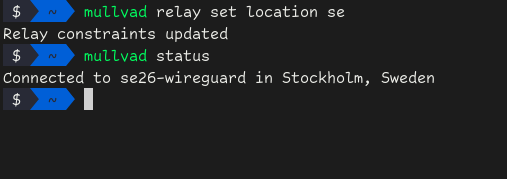
\includegraphics[scale=0.5]{mullvad-status.png}
  \caption{Ändern und Überprüfen des VPN Standorts in der Linux Kommandozeile mit dem \codeinline{mullvad} CLI}
  \label{fig:mullvad-status}
\end{figure}

Die Kommandozeile existiert in zwei Ausprägungen: dem Betriebssystem CLI, auch
als Shell bekannt (siehe die Linux Shell in Abbildung \ref{fig:mullvad-status})
oder der Kommandozeile einer Anwendung (siehe die Node.js Kommandozeile in
Abbildung \ref{fig:node-calc}).

\begin{figure}
  \centering
  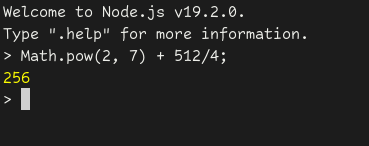
\includegraphics[scale=0.5]{node-calc.png}
  \caption{Durchführung einer Berechnung in der Node.js Kommandozeile}
  \label{fig:node-calc}
\end{figure}

\cite{Spolsky_2001} beschreibt neben der CLI noch zwei weitere Terminal Interfaces welche sich aus diesem entstanden sind:
\\
\textbf{Interaktive CLI}: Ein ``question and answer model'' \parencite[42]{Spolsky_2001} der Kommandozeile, wo der Nutzer mittels Fragen, auf die eine Antwort erwartet wird, entlastet wird. Mehr dazu in Kapitel \ref{chap:interactive}.
\\
\textbf{Menu-driven CLI}: auch als Ncurses CLI bekannt. Das Menü-basierte CLI ähnelt dem GUI indem

% Vergleich zu GUI
% function-orient vs object-oriented vgl. nielson1993

\textbf{Flagge}: Zusammen mit Argumenten sind Flaggen der primäre Weg für eine
CLI App um Werte von Nutzern entgegen zu nehmen \parencite{12factor}. Sie
existieren meist in langer, erkennbar durch die \codeinline{--} am Anfang, oder
kurzer Version, mit nur einem \codeinline{-} und meist dem Anfangsbuchstaben der
Langversion.

\begin{code}
\begin{shellcode}
grep --file FILE
grep -f FILE
\end{shellcode}
\captionof{listing}{Kurze und lange Flaggen am Beispiel equivalenter grep Aufrufe}
\medskip
\end{code}

In dem Beispiel mit grep wird von \codeinline{--file FILE} eine Datei mit
Mustern zum Vergleichen übergeben. Bei mehreren Flaggen ist die Reihenfolge
egal.

\begin{code}
  \begin{shellcode}
  grep --ignore-case
  grep -i
  \end{shellcode}
  \captionof{listing}{Ein Beispiel von Boolean Flaggen}
  \medskip
\end{code}

Die \codeinline{--ignore-case} Flagge von Grep ist eine Boolean Flagge. Meist
wird durch Abwesenheit eine Verneinung ausgedrückt und durch Anwesenheit
\codeinline{true}. Boolean Flaggen übergeben keine Werte sondern ändern das
Verhalten der App. Im Falle von grep's \codeinline{ignore-case} existiert
zusätzliche noch eine \codeinline{--no-ignore-case} Flagge, falls der Nutzer
explizit sein möchte. Kurze Booleanflaggen ermöglichen auch konstrukte
wie dieses: \codeinline{tar -xzf file.tgz}. Es werden die Booleanflaggen
\codeinline{-x}, \codeinline{-z}, wie auch die normale \codeinline{-f FILE}
Flagge kombiniert.

\textbf{Argument}: Argumente erlauben es der CLI Werte von Nutzer anzunehmen.

\begin{code}
  \begin{shellcode}
mv SOURCE DEST
  \end{shellcode}
  \captionof{listing}{Manual Auszug von mv, in seiner simpelsten Form}
  \medskip
\end{code}

Anders als bei Flaggen ist Reihenfolge ausschlaggebend. Beim obigen
\codeinline{mv} Programmaufruf ist das erste Argument die Ausgangsdatei und das
zweite die Zieldatei. Die eigentlichen Dateien unterscheidet nichts, einzig die
Reihenfolge beschreibt die Absicht.

% TODO: Pipe, Interaktive, Menu -> alternative Wege zur Übergabe von Werten

%%% Methoden
\chapter{Entwicklung von Methoden}
% TODO: intro here

\section{Methodologie}
% [Beschreibung des geplanten Vorgehens(-modells) zur Lösung der Problemstellung; umfasst u.a.:

Die Artefakte dieses Kapitels sind die folgenden:
\begin{enumerate}
  \item Eine Auflistung von Problemen welche den Umgang mit Kommandozeilen Interfaces erschweren
  \item Eine Auflistung von Methoden welche diese Probleme adressieren
\end{enumerate}

In Literaturrecherche sollen Probleme erschlossen werden, als auch die dafür -
möglicherweise vielfach - vorliegenden Lösungsansätze. Welche dann, unter Bezug
auf das Problem, als Methoden formuliert dokumentiert werden sollen.
\\
Die Formulierung als Methode soll dabei den Lösungsansatz so beschreiben das
dieser anwendbar ist. Dies ist u.a. erforderlich da die Methoden im nächsten
Schritt angewandt werden sollen.

\section{Probleme mit Kommandozeilen Interfaces}

Es folgen, in nicht priorisierter Reihenfolge, Probleme welche die
Nutzungsschwelle von Kommandozeilen Interfaces erhöhen, d.h. diese weniger
zugänglich.
\\
Diese bestmöglich zu adressieren sollte zu einer Absenkung der Nutzungsschwelle
und damit besser zugänglichen Applikationen führen.

\subsection{Erinnern von Kommandos}

Das Problem des Erinnern von Kommandos (engl. Command recall) beschreibt das
Nutzer sich bei Verwendung eines Programmes an dessen Namen, Kommandos und
Parameter erinnern müssen \parencite{Raskin_2008}.

\fbox{\parbox{\linewidth}{
  \label{prob:command-recall}
  \textbf{Problem~\ref{prob:command-recall}}: Es muss sich an Programmname, Kommandos und Parameter erinnert werden.
}}

Um dieses allgemeine Problem zu adressieren wird es sind kleinere Teilprobleme
aufgespalten.

\medskip

\begin{figure}
  \centering
  
\includegraphics[scale=0.5]{empty-prompt.png}
  \caption{Die Shell bietet nichts an, ohne ein Programm zu kennen passiert nichts.}
\end{figure}

\cite{Gentner_1996} beschreibt auch den Fakt das es keinen einfachen Weg zum
Auffinden von Programmen gibt.
\\
Der Nutzer muss also den Namen des Programmes kennen um dieses zu nutzen.

\smallskip

Unter der Annahme den Names des Programmes zu kennen, geht es nun darum einen
Programmaufruf mit Kommandos und Parametern zusammen zu bauen.
Hierzu können verschiedene Szenarien betrachtet werden.
Der Nutzer:

\begin{enumerate}
  \item hat Kommandos und Parameter auswendig gelernt
  \item baut den Programmaufruf mit Hilfe der Dokumentation zusammen
  \item fügt den Programmaufruf (mit copy-paste) ein
  \item ruft das das Programm indirekt auf (über ein Script oder Alias)
\end{enumerate}

Diese Szenarien sind aber alle nicht ideal:

\medskip

Das 1. Szenario gilt nur mit dem Programm vertraute Nutzer. Und selbst diese
vergessen mit der Zeit. % TODO: citation needed, vergessen

\medskip

Szenario Nummer 2. ist zeitintensiv für den Nutzer. Auch gilt die Annahme das
Dokumentation existiert und das der Nutzer mit dieser umgehen kann.

\medskip

Für Szenario Nummer 3. muss der Nutzer von irgendwo kopieren, die Quelle ist
hier entweder auch die Dokumentation oder externe Portale wie Foren oder
Stack Overflow. In der Dokumentation musst der Programmaufruf auch erstmal
gefunden werden. Und die externen Portale sind für den Bau des Interfaces nicht
verlässlich.

\medskip

Szenario Nummer 4. gilt nur für erfahrene Nutzer die schon mit der Shell
vertraut sind.

\medskip

Es gibt auch Mischformen, wie das der Nutzer Kommando aber nicht Parameter kennt
und dieses nachschaut, diese sind aber in der Betrachtung zu vernachlässigen, da
die Kritiken an den Reinformen auch für sie gelten.

\subsection{Syntax und Semantik}

``Commands and associated parameters must be typed, maintaining the correct
semantic content and syntactic form.'' \parencite[184]{Westerman_1997}

\cite{Gentner_1996} beschreibt die Kommandozeile auch als sehr starr und wenig
Tolerant gegenüber imperfekter Syntax.

\fbox{\parbox{\linewidth}{
  \label{prob:syntax-semantik}
  \textbf{Problem \ref{prob:syntax-semantik}}: Die richtige Syntax and Semantik muss gewährleistet werden.
}}

\bigskip

% TODO: actually semantic error, replace this with syntax mistake, i.e typo or non existant subcommand
Ein Beispiel für fehlerintolerante Syntax am Beispiel von \codeinline{grep}.
Die man page beschreibt die Syntax: \codeinline{grep [OPTION...] PATTERNS [FILE...]}.
Beim schnell-geschehenen Vertauschen von \codeinline{FILE} und \codeinline{PATTERNS}:

\begin{code}
  \begin{shellcode}
grep ./file "[a-z]{3}"
/bin/grep: [a-z]{3}: No such file or directory
  \end{shellcode}
  \captionof{listing}{Fehlerhafte Kommando Syntax bei grep}
  \medskip
\end{code}

Der Bedeutungsgehalt von Kommandos kann an diesem Beispiel dargestellt werden:

\begin{code}
  \begin{shellcode}
git remote add
git add remote
  \end{shellcode}
  \captionof{listing}{Kommando Semantik am Beispiel von git}
  \medskip
\end{code}

Das Kommando \codeinline{git remote} ist zum verwalten von `tracked repositories'.
\codeinline{git add} markiert eine Datei für den nächsten `commit'.
Je nach Kontext haben \codeinline{add} und \codeinline{remote} eine andere Bedeutung.
\codeinline{git remote add} fügt eine neue `repository' hinzu, \codeinline{git
add remote} markiert aber eine Datei mit dem Namen \codeinline{./remote} für den
nächsten `commit'.

\section{Adressierung der Probleme durch Weiterentwicklungen}
\label{sec:weiterentwicklungen}

Ziel dieser Arbeit ist es Methoden zur Adressierung dieser fundamentalen
Probleme innerhalb der Form der Kommandozeile zu beschreiben.

Die meisten Abhandlungen über das Angehen dieser Probleme versuchen aber aus
dieser Form von Interface auszubrechen.

Historisch wurde die grafische Benutzeroberfläche als Lösung für die Probleme
der CLI gesehen \parencite{Norman_2007}. So wurden dem Nutzer die möglichen
Optionen grafisch präsentiert, anstatt diese nachschauen zu müssen. % TODO: vgl. command recall

Es vollzog sich damit ein Wechsel von der Funktions-orientierten
Kommandozeile hin zum Objekt-orientierten GUI \parencite{nielson1993}. Die
Funktions-orientiertheit drückt sich etwa durch die in `single-command' CLI's
häufig vertretene Verb-Nomen Struktur aus. Beispielsweise in \codeinline{rm
file} oder \codeinline{cat file}. In der Objekt-orientierten Welt gehen alle
Aktionen vom Objekt aus. So wird eine Datei in den Papierkorb gezogen (vgl.
\codeinline{rm file}) oder per Doppelklick angezeigt (vgl. \codeinline{cat
file}). Semantische Probleme (wie mit \codeinline{mv} die Reihenfolge
durcheinander zu bringen) sind damit passé. Und von der Textform befreit sind es
auch die in der CLI prävalenten Syntaxfehler.

Aber auch das grafische User Interface hat seine Schwächen. Und diese werden vor
allem `at scale' sichtbar. Die Massen des Internets lassen sich nicht grafisch
darstellen und auch ein volles Email Postfach ist mit nur grafischen Werkzeugen
wenig durchsichtig. \cite{Norman_2007} beschreibt wie Suchmaschinen hier einen
Ausweg bieten. Norman beschreibt die Suchmaschine als `answer engine'. Eine
flexiblere, robustere, getarnte Kommandozeile die mit Rechtschreibfehlern und
Synonymen umgehen kann.

\section{Gesammelte Methoden}
% Methoden beziehen sich direkt auf ein Problem welches adressiert werden soll.

\newcounter{meth}
\newcommand{\methbox}[2]{
  \fbox{\parbox{\linewidth}{
    \refstepcounter{meth}
    \textbf{Methode~\themeth}: #2
    \label{meth:#1}
  }}
}
\newcommand{\methref}[1]{
  Methode~\ref{meth:#1}
}

Anders als erhofft gestaltete sich die Recherche nach Methoden zur Absenkung
der Nutzungsschwelle als schwierig da, wie bereits angesprochen, das GUI oder
eine andere Form von Nutzerinterface oft als Lösung für die Probleme von
Kommandozeilen angeführt wird.

% TODO: ...

%  philosophie/prinzipien

\subsubsection{Natürliche Sprache}
\label{sec:natural-lang}

\cite{Raskin_2008} beschreibt die Kapazitäten linguistischer
Kommandozeilen, welche Normans Konzept der `answer engines' (vgl. Kapitel
\ref{sec:weiterentwicklungen}) ähneln. Diese haben wie der Name schon hergibt
einen Fokus auf menschlicher Sprache.
Ein schönes, genanntes Beispiel von Google Calendar für die Stärke solcher auf
natürlicher Sprache-basierender Interfaces: ``Sunday dinner at 7:30 p.m. with
Asa Jasa.'' Es sind keine Kommandos erforderlich. Das gewünschte wird einfach
in natürlicher Sprache beschrieben. Syntax ist nur insofern relevant, als das
menschliche Sprache ihre eigene Syntax hat.

\medskip

``Recently, there has been a growing movement that sees today's command line
as a human-first text-based UI, rather than a machine-first scripting platform
\parencite{clig}'' \parencite{Schr_der_2021}

\medskip

Die Syntax- und Semantikeinschränkungen des Kommandozeilen Interfaces lassen
eine alleinig `human language' gestützte Anwendung nicht zu. Zumindest nicht
der Reinform des CLI. Als `human-first` User Interface sollte trotzdem
zumindest eine eingschränkte Form natürlicher Spracheingabe unterstützt werden
\parencite{seneviratne2008new}.

\methbox{human_language}{Unterstütze Eingaben in natürlicher Sprache.}

\subsection{Korrigieren von Rechtschreibfehlern}

Diese Methode zeigt eine gewisse Nähe zur Unterstützung der natürlichen
Sprache (Kapitel \ref{sec:natural-lang}). So hob \cite{Raskin_2008} für die
Linguistische Kommandozeile die Verträglichkeit von Rechtschreibfehlern hervor.

Fehlertoleranz im Bezug auf Rechtschreibung würde auch das Problem der zu strikten Syntax % TODO: ref syntax

zum Teil adressieren. Fehlermeldungen und die damit einhergehende Frustration minimieren.
\cite{clig} empfiehlt ganz konkret: ``If the user did something wrong and you can
guess what they meant, suggest it.'' Im Kontrast dazu soll nach der `Do what I
mean' Philosophie der Fehler direkt und ohne Nutzerfeedback ausgebessert werden
\parencite{DWIM}. Was natürlich schneller ist und den Nutzungsflow nicht unnötig
unterbricht. \cite{clig} weißt aber auch darauf hin das eine fehlerhafte Eingabe
neben Rechtschreibfehlern eben auch aus logischen Fehler resultieren kann. Dann
kann das `Do what I mean' zu sehr unerwartetem, gefährlichem Verhalten führen.

\begin{code}
  \begin{shellcode}
heroku pss
 ›   Warning: pss is not a heroku command.
Did you mean ps? [Y/n]:
  \end{shellcode}
  \captionof{listing}{Korrekturvorschlag eines Rechtschreibfehlers nach \cite{clig}.}
  \medskip
\end{code}

\methbox{typos}{Rechtschreibfehler} % TODO: snappy method name, either suggest or neutral, but not correct

\subsection{Interaktive CLI}
% TODO: move this section into definitions

Als Interaktive CLI ist eine solche bekannt die dem Nutzer nach und nach Fragen
stellt, ähnlich einem Formular. Wie bei einem Formular kann neben Freitext kann
dem Nutzer mit Radiobuttons (auswählen von einer Option aus einer Liste) oder
Checkboxen (auswählen mehrerer Optionen aus einer Liste) zum auswählen. % TODO: fix

% TODO: screenshot mit Q&A format

% TODO: extend, reference sources
% bland2007design, Gentner_1996

\subsubsection{Interaktive Frage bei fehlendem Parameter}

% TODO: vgl. Command recall
Man stelle sich folgendes Szenario vor. Eine CLI hat ein Kommando welches einen Parameter erfordert.
Normalerweise erfolgt beim Weglassen der Übergabe dieses Parameters eine Fehlermeldung welche einen Hinweis darauf gibt.

\begin{code}
  \begin{shellcode}
mullvad relay set location

error: The following required arguments were not provided:
    <country>

USAGE:
    mullvad relay set location <country> [ARGS]

For more information try --help
  \end{shellcode}
  \captionof{listing}{Fehlermeldung bei fehlendem Parameter in mullvad (VPN) CLI}
  \medskip
\end{code}

Die CLI weiß aber bereits was der Nutzer tun möchte und könnte anstatt der
Fehlermeldung einen Prompt geben welcher den Nutzer nach den fehlenden
Parametern fragt \parencite{12factor} oder, je nach Kontext, diesem sogar eine
Liste von Vorschlägen geben, um daraus auswählen. Dem Nutzer wird erspart sich
mit der richtigen Syntax und den Vokabeln auseinander zu setzen.

\methbox{interactive_missing_param}{Bei fehlendem Parameter soll interaktiv nachgefragt werden.}

\begin{code}
  \begin{shellcode}
mullvad relay set location
Enter location country code:
  \end{shellcode}
  \captionof{listing}{Prompt welcher direkt nach fehlendem Parameter fragt}
  \medskip
\end{code}

Fairerweise ist zu bemerken das die mullvad CLI dies auch an anderer Stelle
so handhabt, so fragt die CLI bei \codeinline{mullvad account login} nach der
fehlenden Accountnummer.

Negativ an dieser Methode wäre das der Nutzer nicht im gleichen Maße auf die
Möglichkeit einer komplexeren Verwendung des Kommandos hingewiesen wird (so
nimmt das mullvad Kommando aus obigem Beispiel nicht nur Landes- sondern auch
Stadt- und Hostkennungen). Außerdem wird der Programmaufruf ohne den Parameter
in der Shell History gespeichert, was bedeutet bei das bei zurückgehen zu dem
Aufruf der fehlende Parameter immer noch fehlt und ergänzt oder erneut über den
Prompt übergeben werden muss. % TODO: shorten

Beide Punkte sind aber für Einsteiger eher zu vernachlässigen.

\subsection{Menü oder TUI}

% TODO: screenshot
Das Menü oder auch `Text-based user interfaces' ähneln dem GUI dadurch das der
Nutzer seine Optionen visuell präsentiert bekommt und daraus ausgewählen kann.
\\
Da es aber wie die CLI in Terminal lebt werden auch zum darstellen des Menüs
nur Textelemente verwendet. Zur Implementation wird oft die ncurses Bibliothek
verwendet.

\bigskip

Im einem Experiment von \cite{Westerman_1997} hatte das Menü-basierte
Interface, für manche Nutzergruppen, unsignifikant bessere Performance als
ein Kommandozeilen Interface. Auch wurde bei freier Wahl das Menü über alle
Nutzergruppen hinweg doppelt so häufig verwendet.

\methbox{menu}{Biete ein Menü-Interface an.}

% TODO: move

\subsection{Autovervollständigung zum Vorschlagen und Vervollständigen von Kommandos/Flaggen}

Auto-completion in der Kommandozeile beschreibt das Verhalten das bei drücken der
(normalerweise) `TAB' Taste etwas vervollständigt wird.

In der Shell funktioniert dies etwa für Programmnamen und die Pfade von Dateien:
\begin{code}
  \begin{shellcode}
wg # Nutzer drueckt TAB
wget

cat ./note # Nutzer drueckt TAB
cat ./notes.md
  \end{shellcode}
  \captionof{listing}{Autovervollständigung in der Shell}
  \medskip
\end{code}

Bei Programmen kann dies, neben der Vervollständigung von Dateipfaden, auch
Kommandos und Flaggen umfassen.

\begin{figure}
  \centering
  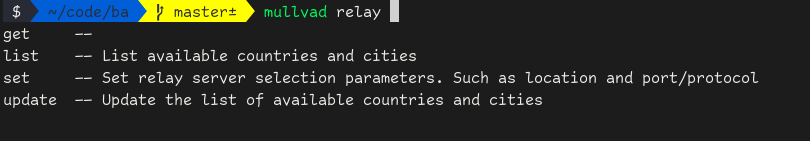
\includegraphics[scale=0.5]{mullvad-autocomplete.png}
  \caption{Bei mullvad's CLI werden nach dem drücken von `TAB' mögliche Kommandos aufgelistet}
  \label{fig:autocomplete}
\end{figure}

% TODO: Vorschlagen beschreiben

\methbox{autocomplete}{Dem Nutzer sollte innerhalb der App Autovervollständigung zu verfügung gestellt werden.}

Auto-completion adressierte beide Probleme welche das CLI mit sich bringt, durch
das Vorschlagen und Vervollständigen erleichtert das Erinnern des gesuchten
Kommandos. Und dadurch das nur valide Kommandos vorgeschlagen werden ist das
einhalten von Syntax- und Semantikregeln erleichtert. Auch profitiert der Nutzer
von Kontext-bezogenen Beschreibungen.

In \cite{dutta} geht der Author sogar noch einen Schritt weiter und empfehlen
das automatische Vorschlagen aller Flaggen und Argumente für ein Kommando,
sodass der Nutzer sich nicht mal anschauen muss was für das Kommando benötigt
wird. So wie vom Author beschrieben ist dies aber nicht in der Shell möglich,
sondern müsste meiner Einschätzung nach eine eigene Kommandozeilen Umgebung
gebaut werden, was nicht im Sinne der Zielstellung dieser Arbeit liegt.

\subsection{Relevante Standardwerte}

Relevante Defaults sind nicht Kommandozeilen spezifisch, können dort aber
wichtiger sein als in grafischen Anwendungen.
\\
Dem Nutzer werden die Möglichkeiten eben nicht zur Auswahl gestellt und dieser
klickt die gewünschte Option an. Sondern ist das Auflisten der Möglichkeiten
i.d.R. ein separater Schritt, losgelöst von der eigentlich beabsichtigten Aktion
(z.B. siehe Abbildung \ref{fig:defaults-demo} oder das mit \codeinline{ls -d}
zuerst die verfügbaren Ordner aufgelistet, um sich dann mit \codeinline{cd
ORDNER} in einen von diesen hineinzubewegen,auch .)
\\
Es greift wieder das fundamentale Problem des `Command Recall' (vgl. Problem
\ref{prob:command-recall}). Den Schritt des Auflistens der Möglichkeiten
(ähnlich wie das Auflisten von möglichen Kommandos) ist ein extra Schritt, außer
der Nutzer kann sich an die gewünschte Option erinnern.

\begin{figure}
  \centering
  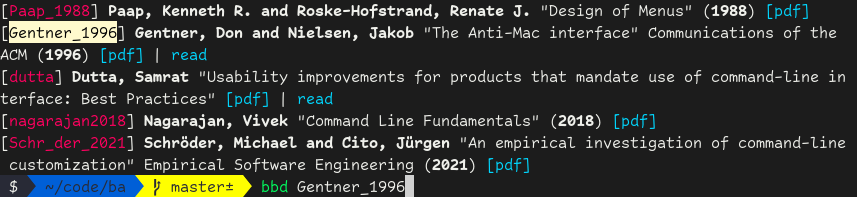
\includegraphics[scale=0.5]{defaults-demo.png}
  \caption{Der erforderte Parameter in dieser Literaturverwaltung ist einer Liste zu entnehmen.}
  \label{fig:defaults-demo}
\end{figure}

\bigskip

\methbox{relevant_defaults}{Falls möglich haben Argumente relevante Defaultwerte.}

Dem Nutzer relevante Standardwerte zu geben erlaubt es diesem weniger
Argumente an die CLI App übergeben zu müssen. Es gibt weniger Fehlermeldungen
die den Nutzer zurückweisen, weil dieser etwas vergessen hat.

Es ist aber auch elementar die Nutzung dieser Standardwerte zu kommunizieren.
Damit der Nutzer von ihnen nicht überrascht wird.

% TODO: describe 12 Factor methods
% https://medium.com/@jdxcode/12-factor-cli-apps-dd3c227a0e46
\subsection{Flaggen anstatt Argumenten}
% 2. Prefer flags to args

Sobald ein Kommando mehr als ein Argument annimmt, biete sich die Gelegenheit
die für Argumente relevante Reihenfolge durcheinander zu bringen (vgl. Command
Recall und Syntax % TODO: fix formating

). \cite{12factor} empfiehlt deshalb bei zwei oder mehr Argumenten Flaggen zu
verwenden. Das ist etwas mehr Aufwand zum Schreiben aber die Reihenfolge als
Fehlerfaktor (vgl. Syntax

) und Flaggen können nun auch mittels Autovervollständigung vorgeschlagen werden
(vgl. \methref{autocomplete}).

\methbox{flags_over_arguments}{Wenn zwei oder mehr Argumenten erforderlich sind nutze stattdessen Flaggen.}

Dies trifft vorallem zu wenn wenn bei dem Kommando schon andere Werte über
Flaggen übergeben werden.

\begin{code}
  \begin{shellcode}
oraclett project add INTPD999DXD --taskDetail "01 - Career development"
oraclett project add --project INTPD999DXD --taskDetail "01 - Career development"
  \end{shellcode}
  \captionof{listing}{Argument ersetzt durch Flaggen: vorher und nachher}
  \medskip
\end{code}

Außen vor sind auch Kommandos welche eine variable Anzahl an Argumenten nehmen,
Beispielsweise \codeinline{rm file1 file2 file3}, weil es sich bei diesen nicht
um verschiedene Typen von Argument handelt \parencite{12factor}.

Ein weiter Vorteil das Erstellen von Aliasen to vereinfachen. Man stelle sich
vor ein App nimmt ein Datum und eine Anzahl von Stunden. Der Nutzer möchte nun
einen Alias der den Tag immer auf heute stellt. Gewünschte Nutzung des Alias sieht so aus:

\begin{code}
  \begin{shellcode}
\$ apptoday 8
  \end{shellcode}
\end{code}

Wenn die App Argumenten nimmt sähe ein Aufruf sowie die Definition des Aliases so aus:

\begin{code}
  \begin{shellcode}
\$ app HOURS DATE

apptoday() {
  app \$1 today
}
  \end{shellcode}
\end{code}

Im Vergleich zu dem Aufruf und Alias mit Flaggen:

\begin{code}
  \begin{shellcode}
\$ app --hour HOURS --date DATE

alias apptoday="app --date today --hour"
  \end{shellcode}
\end{code}

In der Verwendung sind beide equivalent. Beim Schreiben des Alias ist die zweite
Syntax Kommandozeilen Neulingen aber vertrauter, weil man mit dieser zuerst
in Kontakt kommt. Auch ist kein Verständnis von Shell notwendig (hier das
\codeinline{\$1} dem ersten übergebenen Parameter entspricht.)

\subsection{Unterstützung aller Versions- und Helpflaggen}
% 3. What version am I on? -> aliases, get the user what they are looking for

Alle Apps biete eine Hilfs- und eine Versionsseite. Nutzer haben ihre Präferenzen
wenn es darum geht welche Flagge sie verwenden um diese angezeigt zu bekommen.

\begin{code}
  \begin{shellcode}
app -h
app --help
app help

app -v
app -V
app --version
app version
  \end{shellcode}
  \captionof{listing}{Gängige Varianten der Hilfs- und Versionsflaggen}
  \medskip
\end{code}

Laut \cite{12factor} sollten möglichst alle in die App eingebaut sein. So kann
vermieden werden das ein Nutzer nicht das angezeigt bekommt wonach er sucht.

\medskip

\methbox{support_all_help_version}{Unterstütze alle gängigen Formen der Versions- und Helpflaggen.}

\bigskip % TODO: necessary?

\newcommand\checkmark{\ttfamily{\char"2611}}
\newcommand\cross{\ttfamily{\char"2610}}
\begin{table}[h!]
  \begin{center}
    \caption{Unterstützte Varianten von Hilfs- und Versionsflaggen bei einer Stichprobe von 15 Programmen}
    \label{tab:help_version}
    \begin{tabular}{l | c c c | c c c c}
      Programm & \codeinline{-h} & \codeinline{--help} & \codeinline{help} & \codeinline{-v} & \codeinline{-V} & \codeinline{--version} & \codeinline{version} \\
      \hline
git & \checkmark & \checkmark & \checkmark & \checkmark & \cross & \checkmark & \checkmark \\
node & \checkmark & \checkmark & \cross & \checkmark & \cross & \checkmark & \cross \\
mullvad & \checkmark & \checkmark & \cross & \cross & \cross & \cross & \checkmark \\
grep & \cross & \checkmark & \cross & \cross & \checkmark & \checkmark & \cross \\
zathura & \checkmark & \checkmark & \cross & \checkmark & \cross & \checkmark & \cross \\
tsp & \checkmark & \cross & \cross & \cross & \checkmark & \cross & \cross \\
pubs & \checkmark & \checkmark & \cross & \checkmark & \cross & \checkmark & \cross \\
ffmpeg & \checkmark & \checkmark & \cross & \cross & \cross & \cross & \cross \\
systemctl & \checkmark & \checkmark & \cross & \cross & \cross & \checkmark & \cross \\
pacman & \checkmark & \checkmark & \cross & \cross & \checkmark & \checkmark & \cross \\
make & \checkmark & \checkmark & \cross & \checkmark & \cross & \checkmark & \cross \\
synctex & \checkmark & \checkmark & \checkmark & \checkmark & \checkmark & \checkmark & \checkmark \\
curl & \checkmark & \checkmark & \cross & \cross & \checkmark & \checkmark & \cross \\
ansible & \checkmark & \checkmark & \checkmark & \cross & \cross & \checkmark & \cross \\
nvim & \checkmark & \checkmark & \cross & \checkmark & \cross & \checkmark & \cross \\
      \hline
      Summe & 14 & 14 & 3 & 7 & 5 & 12 & 3 \\
    \end{tabular}
  \end{center}
\end{table}

In meinem unrepresentativen Stichprobe stellte sich heraus das
\codeinline{-h} und \codeinline{--help} eigentlich überall funktionieren. Mit
\codeinline{--version} bekommt man in den meisten Fällen auch was man will. Aber
wenn dies nicht zum Ziel führt kommt es zum durcheinander und man muss sich
durchprobieren. Bei ffmpeg gibt es sogar nur eine krude \codeinline{-version}
Flagge.

Am wenigsten verbreitet sind \codeinline{help} und \codeinline{version}, welche
aber auch etwas außen vor sind, weil das erste Argument bei vielen Programmen
eine Input Datei bezeichnet. Aber soweit es die App erlaubt, vor allem bei Apps
mit mehreren Kommandos, sollten auch diese Varianten unterstützt werden.

\subsection{Relevante Kommandovorschläge}

Die Essenz von % TODO: command recall ref

ist das Nutzer nicht wissen welche Kommando oder Subkommando ihnen zur Verfügung
stehen. Kommandos existieren aber nicht im Vakuum. Im Zusammenspiel unterliegen
sie meist einer gewissen Reihenfolge bzw. einem Nutzungs `flow'. Bevor in einen
Ordner gewechselt werden kann (\codeinline{cd}) muss dieser erst existieren
(\codeinline{mkdir}) oder der Nutzer muss von diesem Wissen (\codeinline{ls}).
\cite{dutta} schlägt nun vor sich diesen `flow' zu nutze zu machen um den Nutzer
über mögliche nächste Schritte (in Form anderer Kommandos) zu informieren. In
dem gegebenen Beispiel könnten also \codeinline{mkdir} mit einer Nachricht a là
\codeinline{Also look at - cd, ls} versehen werden. Diese Vorschläge können als
Erinnerung dienen oder den Nutzer dazu Auffordern sich die Vorschläge einmal
näher anzuschauen. Bei `multi-command' CLI's mit vielen Subkommandos, wo der
Nutzer nicht weiß wo er anfangen soll, sind diese Vorschläge besonders wertvoll.

\methbox{command_recommendations}{Schlage dem Nutzer andere relevante Subkommandos vor.}

\chapter{Implementation}
\section{Anforderungsanalyse}
% [Beschreibung der Erhebung, Granularisierung und Priorisierung der zu Grunde liegenden Anforderungen]

Die zu bauende Anwendung wurde konzipiert nicht zu trivial - um genug
Spielraum im Interface Design zuzulassen - aber auch nicht zu komplex - um die
Umsetzbarkeit zu gewährleisten - zu sein.

\subsection{Konzept}
\subsubsection{Problem}

Bei Endava werden die Arbeitsstunden über ein Oracle System festgehalten. Dieses
glänzt nicht in Usability, es führt aber kein Weg dran vorbei.

% TODO: screenshot best case

Das System funktioniert so, dass ein mal wöchentlich die Zeiten der vergangen
Woche abgegeben werden müssen. In diesen Timecards wird angegeben an welchen
Wochentagen man wie viele Stunden an welchem Projekt gearbeitet hat. Bei einem
Projekt und 40 Stunden Woche ist das ausfüllen trivial. Aber sobald man seine
Zeit zwischen mehreren Projekten mit schwankender Stundenzahl aufteilt wird
es komplizierter. Außerdem wird teils gefordert sich Notizen zu machen woran
gearbeitet wurde. Zusammengenommen heißt dies: täglich müssen Dinge bei Oracle
eingetragen werden.

% TODO: screenshot realistic case

\subsubsection{Lösungsansatz}

Die entworfene Lösung ist eine Kommandozeilen App welche das tägliche loggen der
Arbeitszeiten, und Notizen woran gearbeitet wurde, vereinfacht. Und diese Daten
dann zum wöchentlichen Übertragen in Oracle in strukturierter Form ausgibt.
Dadurch wird erreicht nur das erforderliche Minimum der Zeit mit Oracle zu
verbringen, dessen Workflow im übrigen auch am besten funktioniert wenn alles in
einem Rutsch erledigt wird.
\\
Weil es den Rahmen sprengen würde, ohne dem Thema dienlich zu sein, wurde davon
abgesehen die CLI an ggf. bestehende Oracle APIs anzubinden.

\subsection{Anforderungen}

Die Anforderungen wurden in Form von User Stories festgehalten. Erhoben wurden
diese durch den Author in Analyse der eigenen Nutzungsmuster mit Oracle,
abgeglichen in Rücksprache mit anderen Mitarbeitern.

\begin{enumerate}
  \item \textbf{Projekte}:
    \begin{enumerate}
      \item Als Nutzer möchte ich ein Projekt hinzufügen.
      \item Als Nutzer möchte ich einem Projekt einen oder mehrere Task Details anfügen.
      \item Als Nutzer möchte ich die Projekte sowie deren Task Details aufgelistet sehen.
      \item Als Nutzer möchte ich Projekte und Task Details anpassen oder löschen können.
    \end{enumerate}
  \item \textbf{Arbeitszeit}:
    \begin{enumerate}
      \item Als Nutzer möchte ich meine Arbeitsstunden an einem Tag für eine Projekt-Task Detail Kombination loggen.
      \item Als Nutzer möchte ich die geloggten Arbeitsstunden einer gegebenen Woche einsehen.
      \item Als Nutzer möchte ich geloggte Arbeitsstunden anpassen oder löschen.
    \end{enumerate}
  \item \textbf{Arbeitsnotizen}:
    \begin{enumerate}
      \item Als Nutzer möchte ich festhalten woran ich gearbeitet habe.
      \item Als Nutzer möchte ich meine Notizen sehen können.
      \item Als Nutzer möchte ich meine Notizen für einen Tag bearbeiten oder löschen.
    \end{enumerate}
  \item \textbf{Report Generierung}:
    \begin{enumerate}
      \item Als Nutzer möchte ich einen Report für eine gegebene Arbeitswoche generieren, um die Daten in Oracle zu übertragen.
    \end{enumerate}
\end{enumerate}

Diese User Stories sollen einen Eindruck über die Anforderungen der App
und deren Komplexität vermitteln. Das Bauen der App steht aber nicht im
Vordergrund, weshalb u.a. hier die Akzeptanzkriterien der User Stories,
Implementationsdetails wie Datenpersistierung, etc. nicht weiter beschrieben
werden.

\section{Fundament}

Das Fundament der App stellen die zugrundelegenden technologischen Aspekte dar,
welche nicht oder nur indirekt die Nutzbarkeit, und damit den Fokus der Arbeit
betreffen.

Node.js wurde als Programmiersprache gewählt, weil der Author damit vertraut
war, eine Vielzahl von Libraries zum Bauen von CLI's existieren und der
Paketveröffentlichungsprozess mit npm relativ simpel ist. Weiterhin wurden noch
Typescript - für Typisierung - und Eslint - für gleichmäßigen Code Style -
verwendet.

\section{Libraries}

Ein Überblick über die Libraries welche für das Bauen des Interfaces und die
Umsetzung der Methoden relevant waren.

\subsection{oclif}

``oclif is an open source framework for building a command line interface
(CLI) in Node.js. Create CLIs with a few flags or advanced CLIs that have
subcommands.'' \parencite{oclif}

oclif biete ein System um ohne viel Boilerplate Kommandos zu bauen, dessen
Flaggen und Argumente zu beschreiben und dann eigene Businesslogik auszuführen
(siehe Abbildung \ref{fig:oclif-list}.) Während oclif Kommando- und
Flaggenparsing, das generieren der Hilfsseite uvm. übernimmt.

\begin{figure} % TODO: redo, as listing?
  \centering
  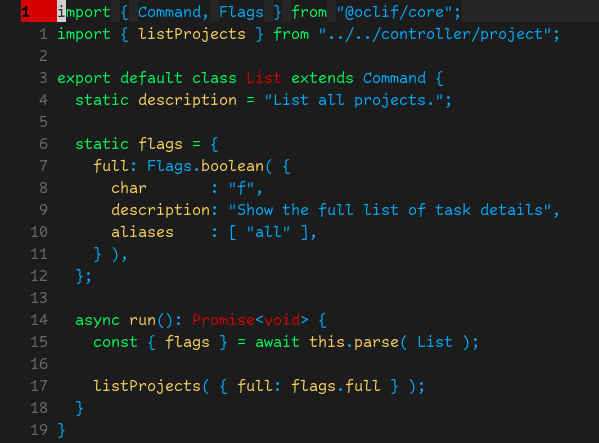
\includegraphics[scale=0.5]{oclif-list.png}
  \caption{Beschreiben eines Kommandos in oclif am Beispiel des implementierten \codeinline{project list} Kommandos}
  \label{fig:oclif-list}
\end{figure}

Die Hierarchie von Kommandos wird über eine Strukurierung der Dateien erreicht (siehe nachstehendes Listing) und der Feinschliff wird noch per Konfiguration in der \codeinline{package.json} erreicht.

\begin{code}
  \begin{shellcode}
 src/commands
 └── project
     ├── add.ts
     ├── edit.ts
     ├── list.ts
     └── remove.ts
  \end{shellcode}
  \captionof{listing}{Kommandohierarchie wird duch Dateistruktur angegeben: Am Beispiel von des \codeinline{project} Kommandos und dessen Subkommandos}
  \medskip
\end{code}

oclif kümmert sich auch um Kleinigkeiten. Zum Beispiel sicherzustellen das der
Text der Hilfsseiten richtig formatiert wird. Im unterstehenden Listing wird
demonstriert wie oclif bei eingeschränkter Breite des Terminals so einrückt
das immer noch klar zu erkennen ist was Beschreibung und was Flagge ist. Das
Gegenbeispiel dazu entsteht wenn einfach nur der Text geschrieben wird, ohne die
Terminalbreite zu berücksichtigen.

\begin{code}
  \begin{shellcode}
# in oclif
FLAGS
  -d, --date=<value>  [default: today] A date to specify the day OR
                      the week (can be human-readable)

# ohne Framework
FLAGS
  -d, --date=<value>  [default: today] A date to specify the day OR
the week (can be human-readable)
  \end{shellcode}
  \captionof{listing}{oclif's Handhabung von Zeilenumbrüchen in einem schmalen Terminal im Vergleich zu einer Implementierung ohne Framework}
  \label{lst:oclif-umbruch}
  \medskip
\end{code}

\medskip

Neben oclif wurde noch andere Frameworks/Libraries in Erwägung gezogen. U.a.
\href{https://github.com/tj/commander.js}{commander.js},
\href{https://github.com/yargs/yargs}{yargs},
\href{https://github.com/dthree/vorpal}{vorpal} und
\href{https://github.com/sindresorhus/meow}{meow}.
\\
In der Sektion \ref{sec:autocomplete} zur Implementation der Autocompletion wird
auch noch auf die Auswirkung der Wahl des Frameworks eingegangen.

\subsection{Inquirer.js}

Inquirer stellt eine komplette Ansammlung an interaktiven % TODO: reference to earlier chapter
Fragetypen zusammen.

Neben einfachen Fragen wie danach Text einzugeben oder aus einer Liste
auswählen, gibt es auch eine Checkbox bei welcher mehrere Einträge einer
Liste gewählt werden können oder einen Prompt zu bearbeiten von Text im
\codeinline{\$EDITOR} (einer Shellvariable in welcher der Nutzer seinen
präferierten Texteditor einträgt).

\begin{figure}
  \centering
  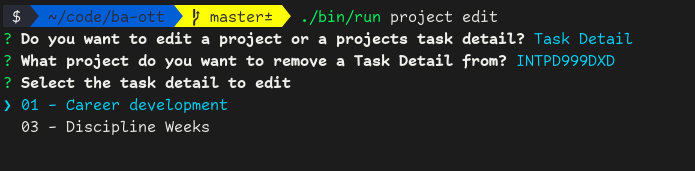
\includegraphics[scale=0.5]{inquirer-example.png}
  \caption{Ein Frage und Antwort Flow zum herausfinden was der Nutzer bearbeiten möchte}
  \label{fig:inquirer-example}
\end{figure}

\begin{code}
  \medskip
  \captionof{listing}{Code Beispiel zum Implementieren eines simplen \codeinline{inquirer list} Prompts}
  \begin{javascriptcode}
const { whatToEdit } = await inquirer.prompt( [ {
  type   : "list",
  name   : "whatToEdit",
  message: "What do you want to edit?",
  choices: [
    {
      name : "Project Name",
      value: "project",
    },
    {
      name : "Task Details (of a project)",
      value: "taskDetail",
    },
  ],
} ] );

// wird zu:

? What do you want to edit? (Use arrow keys)
> Project Name
  Task Details (of a project)
  \end{javascriptcode}
\end{code}

\section{Vorstellung der Implementierten Lösung}

% TODO: how does this chapter look?
% TODO: texts to disjointed?
% TODO: describe npm package

Es folgt eine grobe Vorstellung der Implementierten App. Nachgehend wird
noch einmal seperat auf die Implementation der Methoden zur Absenkung der
Nutzungsschwelle eingegangen.

\medskip

Der Name der App `oraclett' ist kurz für `Oracle time tracker'. Gewählt wurde
dieser weil er 1) kurz und prägnant als auch 2) mit Autovervollständigung leicht
zu finden ist. Intern ist die Platform zu festhalten der Arbeitszeiten als
`Oracle` bekannt, deshalb sollte der Name des Programmes mit \codeinline{oracle}
beginnen damit beim drücken von TAB dann zu \codeinline{oraclett}
vervollständigt wird. Andere in Erwägung gezogene Varianten waren
\codeinline{oracle-time-tracker} oder \codeinline{ott}.

\begin{code}
  \medskip
  \captionof{listing}{Das Hilfsmenu der CLI App}
  \label{code:oraclett-help}
  \begin{shellcode}
  \$ oraclett --help

  Oracle time tracker

  VERSION
    oraclett/0.0.0 linux-x64 node-v19.2.0

  USAGE
    \$ oraclett [COMMAND]

  TOPICS
    hour      Log working hours.
    note      Note down what you worked on.
    project   Add a project code.
    timecard  Generate a report for filling out timecards.

  COMMANDS
    autocomplete  display autocomplete installation instructions
    help          Display help for oraclett.
    timecard      Generate a report for filling out timecards.
  \end{shellcode}
\end{code}

Die Kommandos sind nach dem `noun verb' Prinzip \parencite{clig} strukturiert.
Auf das Nomen, in unserem Fall etwa die Stunde (\codeinline{hour}), folgt
ein Verb wie hinzufügen, bearbeiten, entfernen oder auflisten. Diese Verben
sind bei allen Kommandos einheitlich. Zu bearbeiten eines Projekt wird ebenso
\codeinline{edit} verwendet wie beim bearbeiten einer Notiz.

\begin{code}
  \label{code:hours-help}
  \begin{shellcode}
  \$ oraclett hour --help

  Log working hours.

  USAGE
    \$ oraclett hour COMMAND

  COMMANDS
    hour add     Log working hours.
    hour edit    Edit the logged hours interactively.
    hour list    List all projects.
    hour remove  Remove logged hours interactively.
  \end{shellcode}
  \captionof{listing}{Hilfsseite des `hour' Kommandos}
  \medskip
\end{code}

Die vorgesehene Nutzungsflow wäre wie folgt. Wenn man einem neuen Projekt
zugewiesen wird fügt man dieses \codeinline{oraclett} mit \codeinline{project
add} hinzu.
\\
Im normalen Arbeitsalltag würde man gearbeitete Stunden mit \codeinline{hour
add} festhalten. Auch Notizen dazu woran gearbeitet wurde würden im Moment
selbst mit \codeinline{note add} dokumentiert werden.
\\
Am Ende Arbeitswoche würde mit \codeinline{timecard} ein Report erstellt, dessen
Daten dann in das interne Oracle System übertragen werden. Womit die Woche
abgeschlossen wäre.
\\
Zum Verwalten oder Ausbessern der Daten im System gibt es jetzt noch die
\codeinline{edit} und \codeinline{remove} Subkommandos. Diese stehen falls
benötigt zur Verfügung, sind aber nicht teil des normalen Workflows.

\begin{figure}
  \centering
  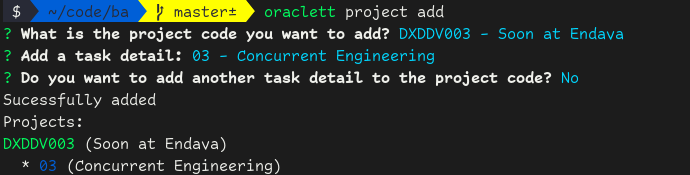
\includegraphics[scale=0.5]{project-add.png}
  \caption{Interaktives hinzufügen eines Projektes.}
  \label{fig:project-add}
\end{figure}

\begin{figure}
  \centering
  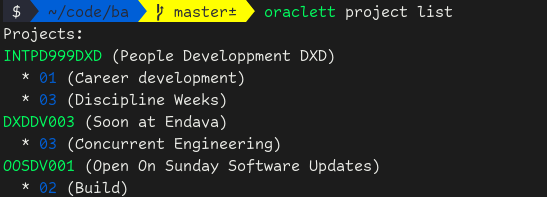
\includegraphics[scale=0.5]{project-list.png}
  \caption{Auflisten der im System vorhandenen Projekte.}
  \label{fig:project-list}
\end{figure}

Die Farben für verschiedene Daten sind einheitlich über alle `list' Kommandos.
So sind die Codes die Referenzcodes Projekte und `Task Details' Grün
bzw. Blau. Dies ist u.a. in den Abbildungen \ref{fig:project-list} und
\ref{fig:note-list} zu sehen. Notizen werden mit Gelb markiert, etwa auf der
Abbildung \ref{fig:note-list}. Und Stundenanzahl sowie Wochentage werden mit
Magenta hervorgehoben, wie zu sehen in Abbildungen \ref{fig:hours-list} und
\ref{fig:timecard}.

\begin{figure}
  \centering
  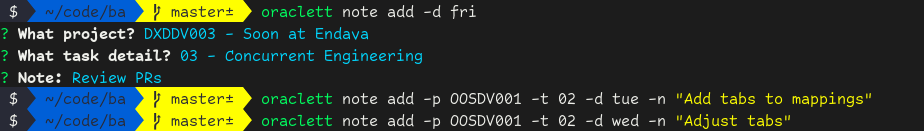
\includegraphics[scale=0.5]{note-add.png}
  \caption{Hinzufügen von Notizen auf interaktivem und normalem Wege.}
  \label{fig:note-add}
\end{figure}

\begin{figure}
  \centering
  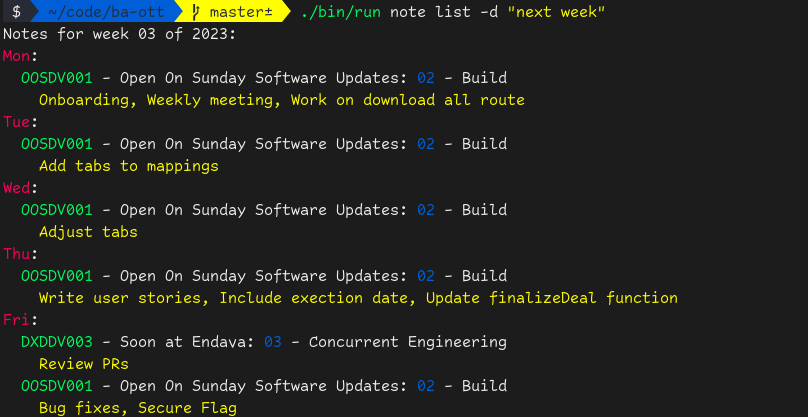
\includegraphics[scale=0.5]{note-list.png}
  \caption{Die Auflistung der Notizen einer gewählten Woche.}
  \label{fig:note-list}
\end{figure}

\begin{figure}
  \centering
  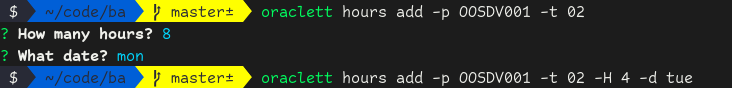
\includegraphics[scale=0.5]{hours-add.png}
  \caption{Loggen von Stunden. Beim Weglassen von Flaggen werden diese interaktiv erfragt.}
  \label{fig:hours-add}
\end{figure}

\begin{figure}
  \centering
  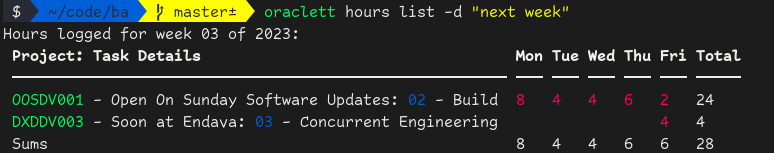
\includegraphics[scale=0.5]{hours-list-real.png}
  \caption{Auflistung der festgehaltenen Stunden.}
  \label{fig:hours-list}
\end{figure}

\begin{figure}
  \centering
  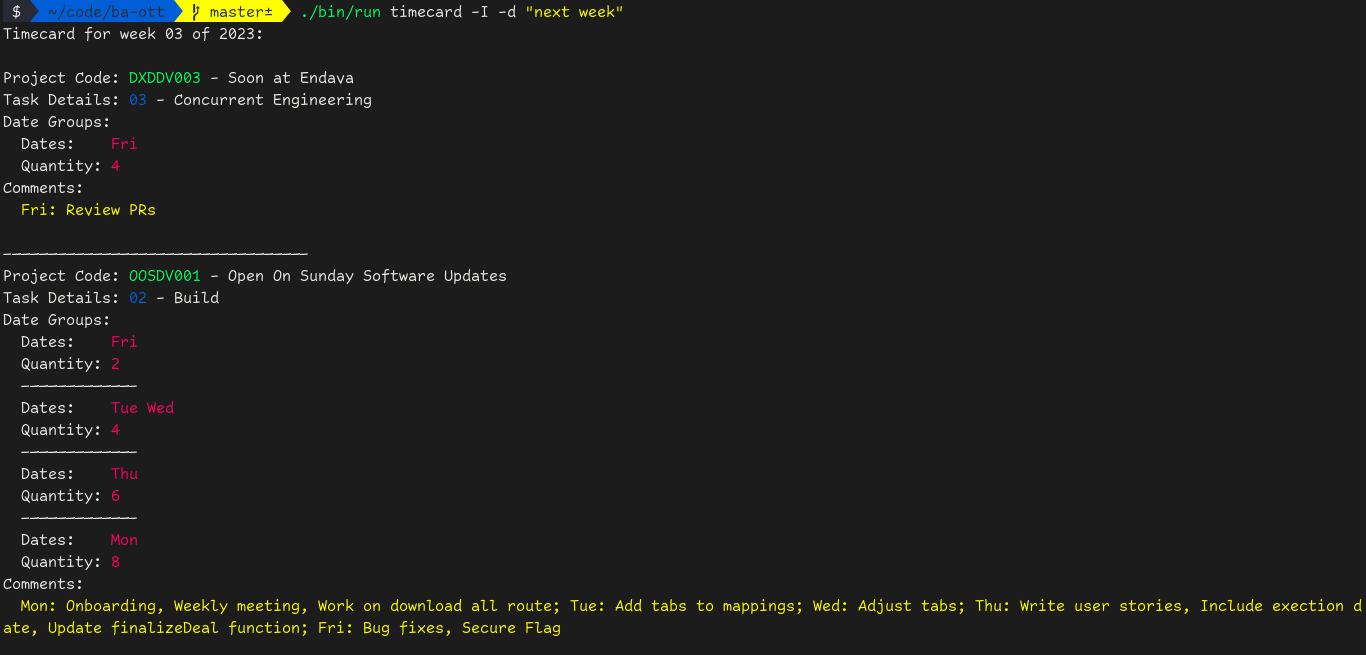
\includegraphics[scale=0.5]{timecard-real.png}
  \caption{Ein die ganze Woche zusammenfassender Report, welcher in seiner Struktur dafür ausgelegt ist in die Web-Oberfläche des internen Tools übertragen zu werden.}
  \label{fig:timecard}
\end{figure}

\section{Anwendung gesammelter Methoden}

Nach dem Verschaffen eines Überblicks, wird nun auf die Anwendung der
gesammelten Methoden näher eingegangen.

\subsection{Relevante Standardwerte}
\label{sec:impl_defaults}

% TODO: methbox nochmal hier?

Die \methref{relevant_defaults} wurde auf zwei Wegen implementiert. Einmal als
exakte Implementation. Und einmal als Weiterführung im Sinne der Methode.

\begin{code}
  \begin{shellcode}
-d, --date=<value>  [default: this week] A date to specify the week (can be human-readable)
  \end{shellcode}
  \captionof{listing}{Die mit default versehene \codeinline{--date} Flagge.}
  \medskip
\end{code}

Obiger Auszug aus dem Hilfsmenü von \codeinline{hour list} kommuniziert das
die \codeinline{--date} Flagge wenn nicht übergeben den Wert \codeinline{this
week} annimmt. Wird das Kommando \codeinline{hour list} ohne Flaggen aufgerufen
werden die Stunden der aktuellen Woche angezeigt. Natürlich kann auch ein
anderer Zeitraum übergeben werden, die aktuelle Woche wird aber am relevantesten
für die meisten Nutzer sein.

\medskip

\begin{figure}
  \centering
  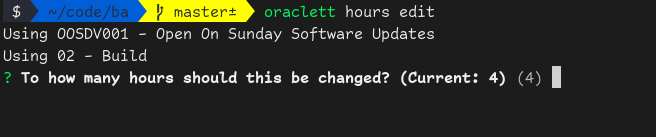
\includegraphics[scale=0.5]{hours-edit-defaults.png}
  \caption{Wenn nur eine Option zur Verfügung steht wird diese automatisch verwendet.}
  \label{fig:hours-edit-defaults}
\end{figure}

Wenn nur eine Option besteht wird diese automatisch gewählt und der Nutzer
darüber informiert. Am Beispiel von \codeinline{hour edit} in der Abbildung
\ref{fig:hours-edit-defaults} sieht das wie folgt aus. Der Standardwert für
das Datum ist \codeinline{today}. Wenn heute nur Stunden für eine einzige
Projekt-Task Detail Kombination festgehalten wurden ist dieses gemeint. Und
am gewählten Tag keine Stunden oder Notizen festgehalten wurden, wird in den
Wochenmodus gewechselt. Dieser erlaubt, wie auch in Abb. \ref{fig:day-week-mode}
zu sehen, das Auswählen eines Wochentages für etwas im System vorliegt.

\begin{figure}
  \centering
  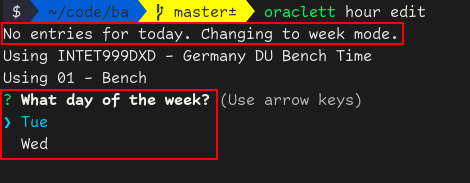
\includegraphics[scale=0.5]{day-week-mode.png}
  \caption{Wechsel vom Tagesmodus, in den Wochenmodus welcher aus Wochentagen mit vorliegenden Daten auswählen lässt.}
  \label{fig:day-week-mode}
\end{figure}

Außerdem wurden eine Auswahl an häufigen geteilten Projekten eingebettet. Der
Nutzer hat immer noch die Möglichkeit diese zu entfernen, aber wahrscheinlich
werden diese von allen Anwendern früher oder später einmal benötigt. Darunter
sind u.a. Projekt Codes zum absolvieren von Tranings, internen Events und der
Bank (keinem kommerziellen Projekt zugeordnet).

\subsection{Unterstützung aller Versions- und Helpflaggen}

Im Bezug auf \methref{support_all_help_version} ist zu sagen das natürlich alle
gängigen Varianten verwendbar sind.

Mit oclif war dies sogar sehr einfach:
\begin{code}
  \begin{javascriptcode}
...
"oclif": {
  "additionalHelpFlags": [
    "-h",
    "help"
  ],
  "additionalVersionFlags": [
    "-v",
    "-V",
    "version"
  ],
  ...
  \end{javascriptcode}
  \captionof{listing}{Konfiguration von Hilfs- und Versionsflaggen für oclif in der \codeinline{package.json}.}
  \medskip
\end{code}

\subsection{Flaggen anstatt Argumenten}

\methref{flags_over_arguments} wurde implementiert. Die Kommandos zum Hinzufügen
von Objekten haben zwischen 2-4 Werten die übergeben werden sollen.

\begin{code}
  \begin{shellcode}
\$ oraclett hour add --help

Log working hours.

USAGE
  \$ oraclett hour add [-t <value>] [-p <value>] [-d <value>] [-H <value>]

FLAGS
  -H, --hour=<value>        The number of hours to log. (1h: 1, 30min: 0.5, etc.)
  -d, --date=<value>        [default: today] The date for which to log (can be human-readable)
  -p, --project=<value>     A project code (it it's short version)
  -t, --taskDetail=<value>  The task details (in it's short version, e.g. 01)

DESCRIPTION
  Log working hours.

  Passing no arguments will start an interactive session.

  This will add to existing hours, if this command is run twice the hours logged will be doubly.

ALIASES
  \$ oraclett hour log

EXAMPLES
  \$ oraclett hour add
  \$ oraclett hour add -H 3
  \$ oraclett hour add -H 3 -p INTPD999DXD -t 01
  \$ oraclett hour add -H 3 -p INTPD999DXD -t 01 --date yesterday
  \$ oraclett hour add -H 10 -p INTPD999DXD -t 01 -d today --force
  \end{shellcode}
  \captionof{listing}{Hilfsmenü von \codeinline{hour add}}
  \medskip
\end{code}

Neben dem Wegfallen der Reihenfolge sind die Flaggen auch elementar für das
Zusammenspiel mit anderen Methoden. Wenn der Nutzer von Defaultwerten Gebrauch
machen oder fehlende Werte interaktiv ergänzen will, kann die spezifische Flagge
einfach weg gelassen werden. Mit Argumenten wäre dies nicht so möglich gewesen.

\subsection{Autovervollständigung}
\label{sec:autocomplete}

Die \methref{autocomplete} und die damit verbundene Autovervollständigung ist
technisch gesehen implementiert, praktisch ist diese aber nicht nutzbar.

\begin{figure}
  \centering
  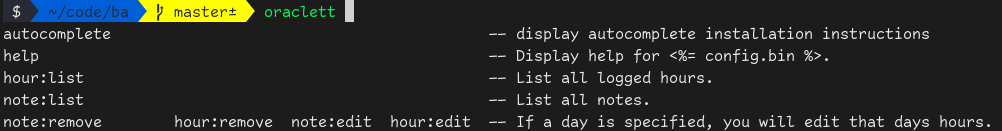
\includegraphics[scale=0.5]{apps-autocomplete.png}
  \caption{Problematisches Autovervollständigungsmenü der App}
  \label{fig:apps-autocomplete}
\end{figure}

Wie auf der Abbildung \ref{fig:apps-autocomplete} zu sehen ist bestehen einige
Probleme. Am offensichtlichsten sind die Doppelpunkte (`:`) zum Trennen
der Kommandos anstatt von Leerzeichen. Dies ist eine Konvention welche
so durch oclif vorgegeben wir (obwohl Leerzeichen viel weiter verbreitet
sind.) In der letzten Zeile wird als Beschreibung etwas von ``If a day is
specified [..]'' geschrieben. Es wurde nicht die Zusammenfassung verwendet
sondern ein Schnipsel aus dem Hilfsmenü. Welcher an dieser Stelle nur
verwirrend für den Nutzer ist. Und zu letzt wird in der Beschreibung der
ersten Zeile der Beginn des Satzes nicht großgeschrieben und in der zweiten
Zeile wird der Template String nicht evaluiert. Alle dieser Dinge sind nicht
konfigurierbar. Für eine ordentliche Vervollständigung müsste diese also
selbst gebaut werden. oclif erschwert dies aber für andere Libraries wie
\href{https://github.com/f/omelette/issues/52}{omelette}. Und die Completion
Dateien selbst in Shell zu schreiben, ohne den Zugriff auf die Quelldateien
welche die Struktur und Inhalte vorgeben, wäre sehr fehleranfällig.
\\
Die geringe Qualität dieser Autovervollständigung war beim initialen Testen
des Frameworks und dem Lesen der Dokumentation nicht ersichtlich. Und nach
der Implementation war es zu spät zu einem anderen Framework zu wechseln, bei
welchem möglicherweise eine bessere Autocompletion möglich gewesen wäre.
\\
Um Verwirrung bei den Endnutzer zu Vermeiden wurde die Funktionalität wieder aus
der App entfernt. Es ist leider enttäuschend von dieser Methode keinen Gebrauch
machen zu können.

\subsection{Fehlende Parameter durch interaktives Fragen ermitteln}

Wie schon in Abbildung \ref{fig:hours-add} zu sehen wurde die
\methref{interactive_missing_param} konsequent implementiert. So ist in der
Abbildung zu sehen wie die fehlenden Stunden- und Datumsangaben erfragt werden.

\medskip

% TODO: besonders das auswähle aus der Liste hervorheben

\subsection{Natürliche Sprache}
\label{sec:sol-natural-lang}

Die \methref{human_language} wurde primär durch die Eingabe von Daten in
natürlicher Sprache implementiert. So kann anstatt starrer Formate wie
\codeinline{MM/DD/YY} einfach \codeinline{Monday} geschrieben werden wenn
der Montag dieser Woche gemeint ist.

\begin{code}
  \medskip
  \captionof{listing}{Unterstützte Varianten der Datumsangabe.}
  \begin{shellcode}
  mon, last monday, monday two weeks ago, today, yesterday, tomorrow, aug 15
  \end{shellcode}
\end{code}

Eingaben wie \codeinline{Monday} oder \codeinline{yesterday} sind
keine absoluten Datumsangaben, sondern steht immer im Kontext dazu wann der
Befehl ausgeführt wird. Da aber der Fokus der Anwendung auf der aktuellen und
vergangenen Woche liegt besteht darin kein Problem (vgl. gewählte Standardwerte
beschrieben in Kap. \ref{sec:impl_defaults}). In der Evaluation zeigten sich die
Nutzer auch zufrieden damit auf diesem Wege Zeitpunkte zu beschreiben. Absolute
Datumsangaben werden aber natürlich auch unterstützt.

\medskip

Auch sollten Synonyme für Subkommandos ``erkannt'' werden. Gedacht war das
Einrichten von alternativen Namen bzw. Aliasen. So sollten Subkommandos
wie \codeinline{hour} auch als \codeinline{hours} erkannt werden. Oder
\codeinline{remove} als \codeinline{delete}, etc. Leider wurde dies von oclif
nur inkonsequenz und verwirrend unterstützt. So können Flaggen ganz einfach mit
einem Alias versehen werden. Auch Kommandos haben diese Option, dabei würde aber
folgendes heraus kommen:

\begin{code}
  \medskip
  \captionof{listing}{Auszug aus dem Hilfsmenü von \codeinline{hour}. Subkommandos \codeinline{add} und \codeinline{log} teilen die gleiche Beschreibung.}
  \begin{minted}[
    linenos,
    numbersep=6pt,
    frame=lines,
    framesep=2mm,
    fontsize=\footnotesize,
    highlightlines={2,5}
  ]{shell}
  COMMANDS
  hour add     Log working hours.
  hour edit    Edit the logged hours interactively.
  hour list    List all logged hours.
  hour log     Log working hours.
  hour remove  Remove logged hours interactively.
  \end{minted}
\end{code}

Kommandos die als Alias markiert sind tauchen immer in den Hilfsseiten auf.
Dadurch wird die Liste weniger übersichtlich. Und der Nutzer weiß nicht was
der Unterschied ist. Es gibt aber von oclif keinen Wege diese zu verstecken.
Wessenwegen sich gegen diese potenziell Frustrationssparenden Aliase entschieden
wurde.

\subsection{Umgang mit Rechtschreibfehlern}

Sehr ähnliche Synonyme wie die in Kap. \ref{sec:sol-natural-lang} genannten
\codeinline{hour} $\leftrightarrow$ \codeinline{hours} können durch die
Fehlerkorrektur verbessert werden (siehe Abbildung \ref{fig:did-you-mean}.)
Weiter entfernte wie \codeinline{remove} $\leftrightarrow$ \codeinline{delete}.

Im Bezug auf \methref{typos}:

\begin{figure}
  \centering
  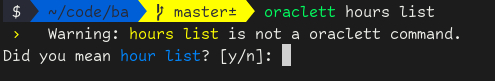
\includegraphics[scale=0.5]{did-you-mean.png}
  \caption{Beispiel der `Meintest du ..' Fehlerkorrektur.}
  \label{fig:did-you-mean}
\end{figure}

\smallskip

Um bei Tippfehler dem Nutzer aber trotzdem einen schnellen Weg zum ausführen
des richtigen Befehls zu geben wurde oclif's Fehlerkorrektur hinzugefügt (siehe
Abbildung \ref{fig:did-you-mean}.)

\subsection{Relevante Kommandovorschläge}

\methref{command_recommendations} hat in der App keine Anwendung gefunden. Wie
auch in der Erklärung wiedergegeben spricht \cite{dutta} diese Empfehlung in
Hinsicht auf CLI's mit sehr vielen (Sub-) Kommandos aus. Die implementierte
Anwendung umfasst nur eine sehr limitierte Anzahl von Subkommandos. Aufgrund
dieser bereits gegebenen Übersichtlichkeit wurde sich gegen direkte Vorschläge
entschieden.

\medskip

In Fehlermeldungen wurde der Geiste der Methode aber angewandt. So verweist ein fehlendes Projekt etwa auf das Hinzufügen und Auflisten von Projekten hin (vgl. Abb. \ref{fig:recommendation-invalid-project}.)

\begin{figure}
  \centering
  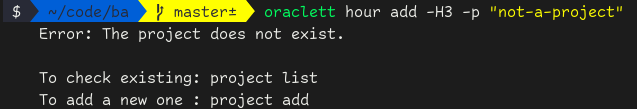
\includegraphics[scale=0.5]{recommendation-invalid-project.png}
  \caption{Vorschläge zum Hinzufügen und Auflisten von Projekten bei Angabe eines Invalides Projektnamens.}
  \label{fig:recommendation-invalid-project}
\end{figure}

\subsection{Menü-basiertes Interface}

Bei der \methref{menu} zum Menü wurde sich gegen eine Implementierung
entschieden. Die Anforderungen hätten aber durchaus als Menü abgebildet werden
können. Das Interface wäre aber von dem Kommandozeilen Interface gänzlich
abgetrennt. Die Implementation und eine über beide Interfaces hinweg eine
konsistente Nutzungserfahrung zu gewährleisten würde einen, im Vergleich zum
Rest der App, unverhältnismäßigen Programmieraufwand mit sich bringen. Weshalb
sich aufgrund des zeitlichen Rahmens dagegen entschieden wurde.

\chapter{Evaluation}
\section{Design der Studie}

Es wurde ein Usability-Test durchgeführt. Laut \cite[36]{henger2003} werden
dabei ``[..] konkrete Nutzungssituationen durch repräsentative Endnutzer
simuliert, um die Bedienbarkeit eines Produkts oder Prototypen zu überprüfen.''
Es wurde die implementierte CLI App der existierenden GUI Webapp gegenüber
gestellt. Die Teilnehmer haben in beiden Apps Aufgabenstellungen erfüllt und
dann die Attraktivität der Applikation bewertet. Das Ziel war es zu sehen
welchen Effekt die entwickelten und implementierten Methoden auf die Nutzbarkeit
der CLI hatten. Ob die, der Kommandozeile inhärente, Nutzungsschwelle abgesenkt
wurde. Die existierende GUI Webapp diente dazu als Maßstab gegen welchen es die
Usability der CLI zu vergleichen galt.

\subsection{Rahmenbedingungen}

Die Teilnehmer der Studie waren ebenso wie der Author Mitarbeiter bei
Endava. Dies ergibt sich daraus das zum Vergleich die Zugriffsrechte für die
GUI Applikation benötigt wurden. Auch wurde die CLI App speziell auf die
Gegebenheiten bei Endava angepasst.

% TODO: number of participants here
Im Rahmen des Usability-Testes wurden x Personen befragt. Laut
\cite[11]{Spolsky_2001} ist ``[..] five or six users [..] all you need.''.
Durchgeführt wurde dieser via Videoanruf mit geteiltem Bildschirm.

% TODO: on user experience level
% Um die Zugänglichkeit zu überprüfen wurden präferiert
% Nutzer mit keinen bis wenig Vorkenntnisse mit der Kommandozeile gewählt.

\subsection{Aufgabenstellungen}
\label{aufgaben}

Es sollten die selben Aufgaben in beiden System erledigt werden. Um dies zu
ermögliche wurde das Spielfeld gleichgestellt. Das heißt das Verwalten von
Projekten in der CLI wurde ausgeklammert weil dies in der GUI vom System
verwaltet wird. Auch wurde das Erstellen von Reports zum Übertragen von CLI in
GUI außen vor gelassen.
\\
Die Teilnehmer werden das erste Mal mit der CLI App gearbeitet haben. Den
Nutzern sollte genung Zeit gegeben werden um mit der Anwendung vertraut zu
werden und diese zu erlernen. Auf Anratens von Prof. Israel wurde deshalb eine
Menge von 20 Aufgaben gewählt.
\\
Die Studie wurde auf Englisch durchgeführt. Deshalb sind die Aufgaben hier auch
im orignalen Wortlaut wiedergegeben.

\begin{enumerate}
  \item Add 8 hours for today on the Bench (INTET999DXD - Germany DU Bench Time / 01 - Bench)
  \item Describe that you worked on "Self-Learning" during that time today (INTET999DXD - Germany DU Bench Time / 01 - Bench)
  \item Add another 8 hours for tomorrow on the Bench (INTET999DXD - Germany DU Bench Time / 01 - Bench)
  \item Change the 8 hours for tomorrow to 6 (INTET999DXD - Germany DU Bench Time / 01 - Bench)
  \item Remove the 6 hours for tomorrow (INTET999DXD - Germany DU Bench Time / 01 - Bench)
  \item Log 2 hours on the Bench for Friday this week (INTET999DXD - Germany DU Bench Time / 01 - Bench)
  \item Add 6 hours on "People Development - Certification" for Friday this week (INTPD999DXD - People Development DXD / 02 - Certification)
  \item Describe that you did a "Node.js Certificate" in the hours you just logged (INTPD999DXD - People Development DXD / 02 - Certification)
  \item Change todays 8 hours on the bench to 2 (INTET999DXD - Germany DU Bench Time / 01 - Bench)
  \item And delete your note ("Self-Learning") for today (INTET999DXD - Germany DU Bench Time / 01 - Bench)
  \item Add 4 hours of Dev Discipline for today (INTDS999DXD - Endava Disciplines DXD / 08 - Team Development)
  \item Add 4 hours of Testing Discipline for today (INTDS999DXD - Endava Disciplines DXD / 12 - Team Testing)
  \item Add 3 hours of both Testing Discipline and Dev Discipline for Monday of this week (INTDS999DXD - Endava Disciplines DXD / 08 - Team Development + 12 - Team Testing)
  \item Log 6 hours on the bench for Monday, Tuesday and Wednesday of next week (INTET999DXD - Germany DU Bench Time / 01 - Bench)
  \item Add a note for Monday of next week that you "Played around with Golang" (INTET999DXD - Germany DU Bench Time / 01 - Bench)
  \item Change the just added note to "Played around with Rust" (INTET999DXD - Germany DU Bench Time / 01 - Bench)
  \item Change the hours for next weeks Tuesday and Wednesday to 8 (INTET999DXD - Germany DU Bench Time / 01 - Bench)
  \item Delete the hours logged for next weeks Wednesday (INTET999DXD - Germany DU Bench Time / 01 - Bench)
  \item Show and tell Jonathan how many hours you worked in total for this week
  \item Show and tell Jonathan how many hours you logged for the Bench next week
\end{enumerate}

Das Hinzufügen zum System spielt die Hauptrolle. In der echten Verwendung wäre
das \codeinline{add} Kommando auch das meist verwendete.

Die Anzahl von Aufgaben welche pro Kommando erledigt werden:
\begin{itemize}
  \item 8: \codeinline{hour add}
  \item 3: \codeinline{note add}
  \item 3: \codeinline{hour edit}
  \item 2: \codeinline{hour remove}
  \item 2: \codeinline{hour list}
  \item 1: \codeinline{note edit}
  \item 1: \codeinline{note remove}
\end{itemize}

Um das Spielfeld etwas zu ebnen stimmen die Verben zum Beschreiben was getan
werden soll nicht immer mit den Verben die in der CLI App verwendet werden über.
So verwenden beispielsweise die 18. Aufgabe das Wort `delete' anstatt `remove',
die 2. nutzt `describe' anstatt `add', die 4. `change` statt `edit' und 6. `log'
anstatt `add'. Die Sätze meinen immer noch das selbe, zwingen die Teilnehmer
aber sich an die Name der Kommandos zu Erinnern.

Auch sind z.B. Aufgabe 13. und 14. so gestaltet das diese Aufgrund der unterschiedlichen
Einschränkungen der beiden User Interfaces mit dem einen oder anderen einfacher
zu erledigen seien sollten.

\subsection{Erhobene Daten}

Um die Performance zu messen wurde aufgezeichnet wie lange ein Benutzer
benötigt um eine gegebene Aufgabe zu erfüllen. Dazu wurden die Test Sitzungen
aufgezeichnet und dannach die Zeitmarken von Beginn und Beendung einer Aufgabe
notiert.

Einschätzung der Attraktivität beider Oberflächen erfragt. Wie auf Abbildung
\ref{fig:survey-values} zu sehen ist, bewerten die Teilnehmer die Apps auf einer
Skala zwischen zwei Adjektiven.

\begin{figure}
  \centering
  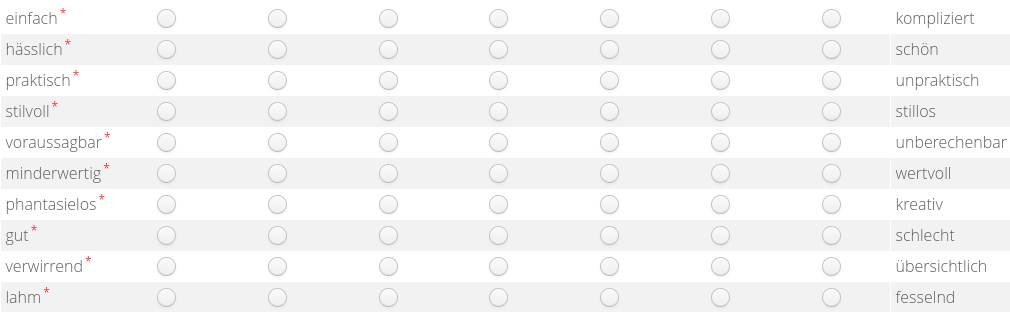
\includegraphics[scale=0.5]{survey-values.png}
  \caption{Beurteilungsbogen der kurzen AttrakDiff Studie}
  \label{fig:survey-values}
\end{figure}

\subsection{Hypothesen}

\newcounter{hypo}
\newenvironment{hypo}[1][]{
  \refstepcounter{hypo}
  Hypothese \thehypo:#1
  \label{hypo:\thehypo}
}

% TODO: Erörtern was Vorstellung, warum Hypothese relevant
Diese Hypothesen sollen durch die erhobenen Daten adressiert werden.

% TODO: style w/ label

\begin{hypo}{Die CLI hat im Durchschnitt eine ähnliche Performance wie die GUI.}\end{hypo}
\begin{hypo}{Die Performance der CLI verbessert sich im Verlaufe des Tests.}\end{hypo}
\begin{hypo}{Die CLI wird der GUI subjektiv vorgezogen.}\end{hypo}

% TODO: rework
Hypothese \ref{hypo:1} bewertet die Performance Unterschiede zwischen den beiden
Applikationen.

Hypothese \ref{hypo:2} soll Erlernbarkeit bewerten. Den Teilnehmer wurde ja
durch die Anzahl der Aufgaben genug Zeit gegeben sich mit der App vertraut zu machen.

Die \ref{hypo:3}. Hypothese bezieht sich auf das Gefühl der Teilnehmer  % TODO: finish

\subsection{Durchführung}

Nach einer generellen Einführung und Installation der App auf der Maschine des
Teilnehmers begann der Teilnehmer entweder mit der GUI Webapp oder der CLI
Applikation. 50\% der Teilnehmer begannen mit der einen, die andere Hälfte mit
der anderen. Vor der Verwendung der CLI App gab es eine Einführung, welche
dazu diente den Teilnehmer mit dem System und dessen Möglichkeiten vertraut
zu machen. Als Ausgleich dafür das die Teilnehmer alle schon mit der GUI
Variante vertraut waren. Mit dem Hinweis darauf, dass der Versuchsleiter keine
Hilfestellung leisten würde, ging es mit der Bearbeitung der Aufgaben los.
Die Checkliste der Aufgaben waren eine nach der anderen zu bewältigen. Nach
Erledigung der Aufgaben folgte die Attraktivitätsumfrage, gefolgt von der
Bearbeitung derselben Aufgaben im anderen System, sowie erneuter Umfrage.

\section{Auswertung}

%%% Finish
\chapter{Zusammenfassung}
% [Aggregierte retrograde Kurzbeschreibung der Arbeit]
\section{Schlussfolgerungen}
% [Beschreibung der insgesamt zu konstatierenden Schlussfolgerungen im Zusammenhang mit der Arbeit]
\section{Limitationen}
% [Beschreibung der Ergebnisse einer kritischen Reflektion und Begr\"undung dessen, was die Arbeit nicht zu leisten vermag]
\section{Ausblick}
% [Beschreibung und Begr\"undung potenzieller zuk\"unftiger Folgeaktivit\"aten im Zusammenhang mit Ihrer Arbeit (z.B. weitere Anforderungen, Theoriebildung, ... ]

\subsection{Erarbeitung weiter Methoden}

Mit mehr Zeit hätten sich weitere Methoden formulieren lassen.
% TODO: hier andere Methoden to look into

\subsection{Strukturierung und Zugänglichkeit der Methoden}

Die Methoden könnten in stärker strukturierter Form und außerhalb des Kontextes
dieser Arbeit für sich stehend formuliert werden. Zusammen mit einer englischen
Übersetzung wären sie dadurch dann leichter referenzier- und implementierbar.

\subsection{Verbesserung der Implementation}

Die konkrete Implementierung hat noch einige Schwächen. So gibt es Dopplungen in
den Hilfsmenüs (etwa \codeinline{timecard} in Listing \ref{code:oraclett-help}
oder \codeinline{hour add/log} in Listing \ref{code:hours-help}), inakkurate
Hilfstexte in der Autovervollständigung oder im \codeinline{oraclett --help}
Menü sowie das die Autocompletion erst durch den Nutzer konfiguiert werden
muss. Diese Probleme sind der Nutzung des ocli Frameworks geschuldet. Es gibt
Möglichkeiten diese zu Adressieren, das war aber im Rahmen dieser Arbeit nicht
möglich.
% TODO: reference to autocomplete implementaton

Eine Anbindung an Oracle selbst war im Rahmen dieser Arbeit nicht vorgesehen,
weil der Fokus auf den Methoden lag. Als zukünftige Verbesserung der App wäre
dies aufgrund der Zeitersparnis aber sinnvoll.

Eine vollständige Implementierung der Methoden \ref{meth:menu} und
\ref{meth:autocomplete} wäre sinnvoll.

%%% possible modules
% \section{Kontext}
% \subsection{Domain}
% \subsection{Technologien}
% \subsection{Methoden und Konzepte}
% \section{...}
% \subsection{...}
% \subsection{...}
% \chapter{Anforderungserhebung und -analyse}
% \section{Nutzer- und Systemanforderungen}
% \subsection{Funktionale Anforderungen}
% \subsubsection{Obligatorisch (MUSS)}
% \subsubsection{Fakultativ (Kann)}
% \subsection{Nicht-funktionale Anforderungen}
% \subsubsection{Obligatorisch (MUSS)}
% \subsubsection{Fakultativ (Kann)}
% \section{...}
% \chapter{Konzeption \& Entwurf}
% [Beschreibung des Entwurfs auf Basis der Methodologie / der geplanten Vorgehensweise zur Probleml\"osung im Kontext der Anforderungen (i.A. der Art der Arbeit)]
% \section{Prozess}
% \section{Systemarchitektur}
% \section{Softwarearchitektur}
% \section{Schnittstellen}
% \section{Datenmanagement}
% \section{...}
% \chapter{Implementierung}
% [Beschreibung der Implementierung\footnotemark auf Basis des Entwurfs und der Methodologie / der geplanten Vorgehensweise zur Probleml\"osung im Kontext der Anforderungen. Hier ist Raum f\"ur Listings, wie z.B. das nun Folgende: Umfangreicher Quell-Code sollte in den Anhang ausgelagert werden.]
% \chapter{Test}
% [Beschreibung, wie Sie auf Basis des geplanten Testvorgehens was mit welchen Kriterien und Technologien getestet haben]
% \chapter{Darstellung und Bewertung der Ergebnisse}
% [Beschreibung der Ergebnisse aus allen voran gegangenen Kapiteln sowie der zuvor generierten Ergebnisartefakte mit Bewertung, wie diese einzuordnen sind]

% \bibliographystyle{apalike}
% \bibliographystyle{ksfh_nat} % ein anderer Stil
% \bibliography{science}
\printbibliography[
heading=bibintoc,
title={Quellenverzeichnis}
]

\newpage
\chapter{Glossar}
\begin{appendix}
\pagenumbering{Roman}
\chapter{Appendix}

\section{Quell-Code}

\section{Tipps zum Schreiben Ihrer Abschlussarbeit}

\begin{itemize}
\item Achten Sie auf eine neutrale, fachliche Sprache. Keine \glqq{}Ich\grqq{}-Form.
\item Zitieren Sie zitierf\"ahige und -w\"urdige Quellen (z.B. wissenschaftliche Artikel und Fachb\"ucher; nach M\"oglichkeit keine Blogs und keinesfalls Wikipedia.
\item Zitieren Sie korrekt und homogen.
\item Verwenden Sie keine Fu{\ss}noten f\"ur die Literaturangaben.
\item Recherchieren Sie ausf\"uhrlich den Stand der Wissenschaft und Technik.
\item Achten Sie auf die Qualit\"at der Ausarbeitung (z.B. auf Rechtschreibung).
\item Informieren Sie sich ggf. vorab dar\"uber, wie man wissenschaftlich arbeitet bzw. schreibt:
\begin{itemize}
\item Mittels Fachliteratur\footnote{Z.B. \autocite{balzert2011}, \autocite{franck2013}}, oder
\item Beim Lernzentrum\footnote{Weitere Informationen zum Schreibcoaching finden sich hier: \url{https://www.htw-berlin.de/studium/lernzentrum/studierende/schreibcoaching/}; letzter Zugriff: 13 VI 19.}.
\end{itemize}
\end{itemize}

\newpage
\thispagestyle{empty}
\noindent

\section*{Eidesstattliche Versicherung}
Hiermit versichere ich an Eides statt durch meine Unterschrift, dass ich die vorstehende Arbeit selbstst\"andig und ohne fremde Hilfe angefertigt und alle Stellen, die ich w\"ortlich oder ann\"ahernd w\"ortlich aus Ver\"offentlichungen entnommen habe, als solche kenntlich gemacht habe, mich auch keiner anderen als der angegebenen Literatur oder sonstiger Hilfsmittel bedient habe. Die Arbeit hat in dieser oder \"ahnlicher Form noch keiner anderen Pr\"ufungsbeh\"orde vorgelegen.\\
\linebreak[4]
\linebreak[4]
\linebreak[4]
\linebreak[4]
-------------------------------------------------------\linebreak[4]
Datum, Ort, Unterschrift

\end{appendix}
\end{document}
